\documentclass[11pt, oneside]{article} 
\usepackage{geometry}
\geometry{letterpaper} 
\usepackage{graphicx}
	
\usepackage{amssymb}
\usepackage{amsmath}
\usepackage{parskip}
\usepackage{color}
\usepackage{hyperref}

\graphicspath{{/Users/telliott_admin/Tex/png/}}
% \begin{center} 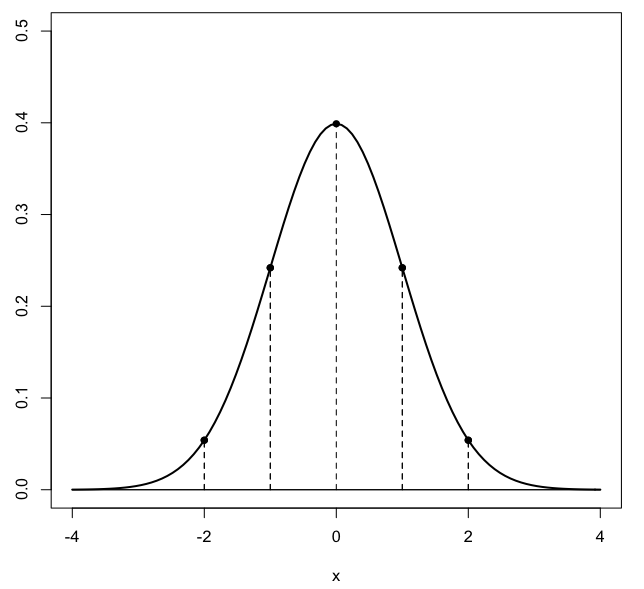
\includegraphics [scale=0.4] {gauss3.png} \end{center}

%break
\title{Exponential and Logarithm}
\date{}

\begin{document}
\maketitle
\Large

In more advanced treatments (analysis), what they do is to investigate a particular function which we will call $L$, and show that the function $L$ has all the properties of the logarithm, \emph{so it is the logarithm}.  

We follow that path here, and then after that go backwards from the logarithm to the other properties of $e$, like its numerical value, and the fact that the derivative of $e^x$ is $e^x$ itself.

This approach comes straight from David Jerrison's lecture in Calculus 1 (MIT online course).  We define the logarithm function as
\[ L(x) = \int_1^x \frac{dt}{t} \]
\begin{center}
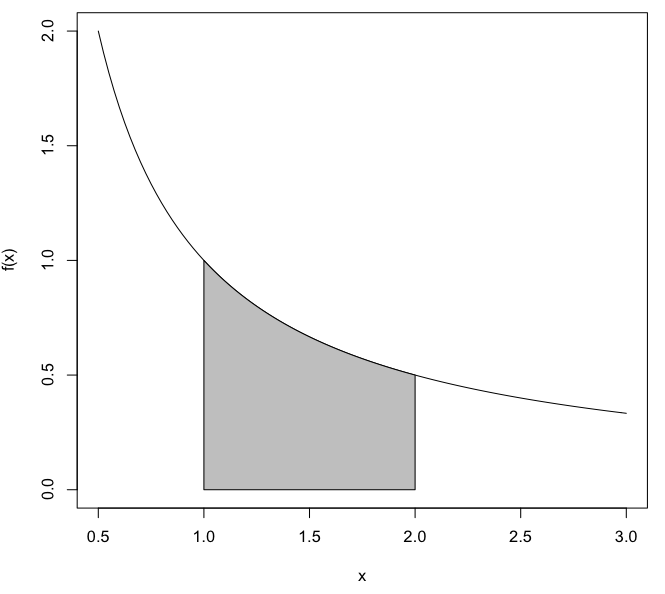
\includegraphics [scale=0.30] {inv.png}
\end{center}
For example, the logarithm of $2$ is the area under the curve above, $f(x) = 1/x$, between $ 1 \le x \le 2$.  Having defined
\[ L(x) = \int_1^x \frac{dt}{t} \]

By the Fundamental Theorem of Calculus (part II) we have

$\bullet  $ Property 1
\[ L'(x) = \frac{1}{x} \]
The slope of the logarithm function is always positive ($x>0$), but is undefined for $x=0$
\begin{center}
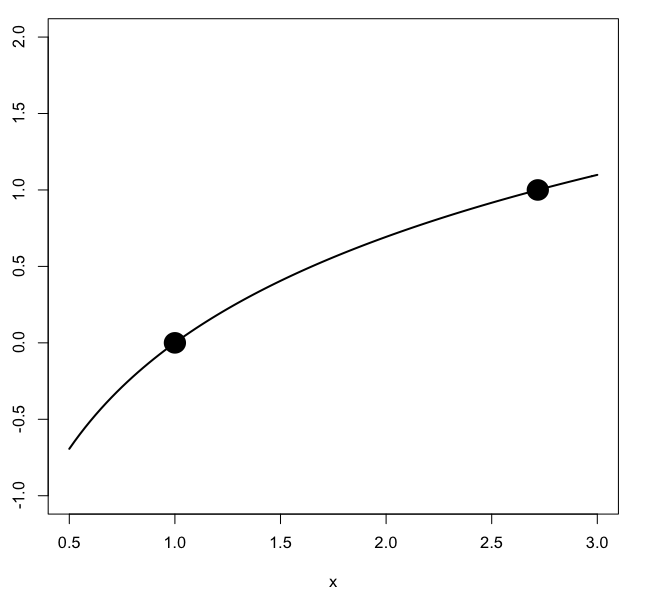
\includegraphics [scale=0.30] {log.png}
\end{center}

$\bullet  $ Property 2
\[ L(1) = \int_1^1 \frac{dt}{t} = 0 \]
This property is by definition.  It fits with our use of exponents, where $b^0 = 1$.

$\bullet  $ Property 3
\[ L''(x) = - \frac{1}{x^2} \]
Although the area under the curve $ln(x)$ is always increasing, so the slope is always positive, the rate of increase of the slope is always decreasing, so the shape is concave down.

$\bullet  $ Property 4
\[ L(e) = 1 \]
This is by definition as well.  In extending to exponents it means $x$ is a single-valued function of $y$, so we can write $y = L(x) \iff e^y = x$.

$\bullet  $ Property 5
\[ L(ab) = L(a) + L(b)  \]
To show that this last statement is true involves showing that
\[ \int_1^{ab} \frac{dt}{t} = \int_1^{a} \frac{dt}{t} + \int_a^{ab} \frac{dt}{t} \]
is both true and equivalent to the first statement.

For the arguments $a$ and $ab$ we have 
\[ L(ab) = \int_1^{ab} \frac{dt}{t}   \]
\[ L(a) = \int_1^{a} \frac{dt}{t}   \]
Both of these are true by definition.  The one that takes a little work is
\[ L(b) = \int_a^{ab} \frac{dt}{t}   \]

We do a substitution.  Let $au=t$, then $a \ du = dt$ and
\[ L(b) = \int \frac{a \ du}{au} = \int \frac{du}{u}  \]

At this point we run into a new idea.  When we change the variable we also must change the bounds.  At the first one, we have $t = a$ so
\[ u = \frac{t}{a} = \frac{a}{a} = 1  \]
At the upper bound, we have $t = ab$ so
\[ u = \frac{t}{a} = \frac{ab}{a} = b  \]

The integral $\int_a^{ab}$ becomes $\int_1^{b}$ and we have
\[ L(b) = \int_1^b \frac{du}{u}  \]
which is again, true by definition.  

Thus, the function $L$ has the property that
\[ L(ab) = L(a) + L(b) \]
which is one of the two major properties of logarithms.

$\bullet  $ Property 6

To see that the second property is also true, start with
\[ L(a^r) = \int_1^{a^r} \frac{dt}{t}   \]
Substitute $t=u^r$, so $dt = ru^{r-1} du$.  The bounds are changed as follows ($r$ can be anything):
\[ t = 1, \ \ \ \  t = u^r \rightarrow  u= 1  \]
\[ t = a^r, \ \ \ \   t = u^r \rightarrow  u = a  \]
This gives
\[ L(a^r) = \int_{t=1}^{t=a^r} \frac{dt}{t} \]
\[ = \int_{u=1}^{u=a} \frac{1}{u^r} (ru^{r-1}) du \]
\[ = r \int_{1}^{a}  \frac{du}{u} = rL(a) \]

That is
\[ L(a^r) = rL(a) \]

As Dunham says (using A for L) 
\begin{quote}"these properties of the hyperbolic area---namely $A(ab) = A(a) + A(b)$ and $A(a^r) = rA(a)$---exactly mirror the corresponding properties of logarithms.  Clearly something interesting is afoot."\end{quote}

\subsection*{Difference quotient for logarithm}
As seen in Hamming, we can also go back to the definition of the logarithm as the inverse of the exponential
\[ f(x) = \log_b x \]
write the difference quotient
\[ f'(x) = \lim_{h \rightarrow 0}  \frac{\log_b (x + h) - \log_b x}{h}  \]
and then use the properties of logarithms to rearrange it as follows:
\[ =  \lim_{h \rightarrow 0} \frac{\log_b (\frac{x+h}{x})}{h} \]
\[ =  \lim_{h \rightarrow 0} \frac{\log_b (1 + \frac{h}{x})}{h} \]
\[ =  \lim_{h \rightarrow 0} \log_b \ [ \ (1 + \frac{h}{x})^{1/h} \ ]  \]
\[ =  \lim_{h \rightarrow 0} \frac{1}{x}  \ [ \ \log_b (1 + \frac{h}{x})^{x/h}  \ ]  \]
Finally
\[ =   \frac{1}{x}  \ \lim_{h \rightarrow 0}  \ [ \ \log_b (1 + \frac{h}{x})^{x/h}  \ ]  \]

So it's clear that we will need to evaluate the term for which we are taking the logarithm, in the limit
\[ =  \lim_{h \rightarrow 0} (1 + \frac{h}{x})^{x/h} \]
Let $t = h/x$.  Then this becomes
\[ =  \lim_{t \rightarrow 0} (1 + t)^{1/t} \]

which ought to look familar from previous chapters.  It is one of the definitions of $e$.  We have then that
\[ \frac{d}{dx} \log_b x = \frac{1}{x} \ \log_b e \]
If we use the natural logarithm, then we have
\[ \frac{d}{dx} \ln x = \frac{1}{x} \ \ln e = \frac{1}{x} \]

There is another derivation which is essentially identical to this one in videos on Khan Academy.

\end{document}